\subsection{At Viking Lander 1 (VL1)}
Figure \ref{fig:sub:comparative-global-insolation-at-vl1-beta-optimal-daily-variations} shows that calculated values are consistently lower than those published in \citemarsenv{Appelbaum1993}. Both daily variations closely follow the same pattern. Figure \ref{fig:sub:comparative-global-insolation-at-vl1-beta-optimal-percentage-differences} reveals that the differences between calculated and published values range between \SI{2}{\percent} and \SI{2.8}{\percent}. Differences larger than \SI{2.5}{\percent} are more frequent for large tau values starting from 1.9.

\begin{figure}[H]
\captionsetup[subfigure]{justification=centering}
\vspace{-2ex}
\centering
    %% setup sizes
    \setlength{\subfigureWidth}{0.50\textwidth}
    \setlength{\graphicsHeight}{80mm}
    %% kill hyper-link highlighting
    \hypersetup{hidelinks=true}%
    %% the figures
    \begin{subfigure}[t]{\subfigureWidth}
        \centering
            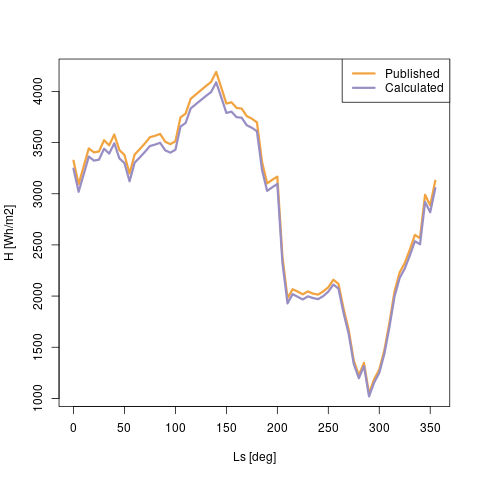
\includegraphics[height=\graphicsHeight]{sections/appendix/A/plots/h-exp-calc-at-vl1-with-beta-65-deg.png}
            \subcaption{Daily variations.}
            \label{fig:sub:comparative-global-insolation-at-vl1-beta-optimal-daily-variations}
    \end{subfigure}\hfill
    \begin{subfigure}[t]{\subfigureWidth}
        \centering
            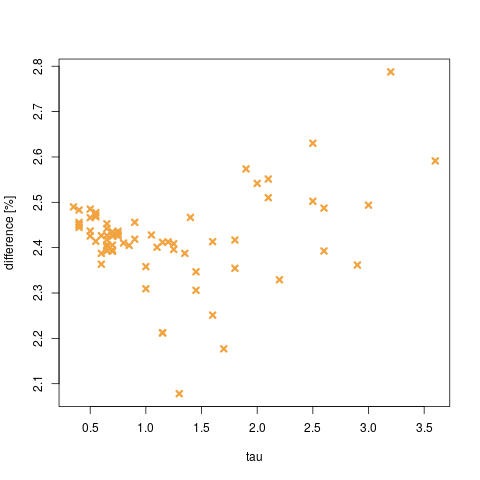
\includegraphics[height=\graphicsHeight]{sections/appendix/A/plots/h-diff-bet-exp-calc-at-vl1-with-beta-65-deg.png}
            \subcaption{Differences as a function of optical depth.}
            \label{fig:sub:comparative-global-insolation-at-vl1-beta-optimal-percentage-differences}
    \end{subfigure}\\[0.8ex]
    \caption{Comparison between published and calculated daily global insolations at \ac{VL1} on a inclined surface with $\beta=\SI{6.5}{\degree}$.}
    \label{fig:plot:comparative-global-insolation-at-vl1-beta-optimal}
\vspace{-2ex}
\end{figure}

\subsection{At Viking Lander 2 (VL2)}
Figure \ref{fig:sub:comparative-global-insolation-at-vl2-beta-optimal-daily-variations} shows that calculated values are consistently lower than those published in \citemarsenv{Appelbaum1993}. Both daily variations closely follow the same patterns. Figure \ref{fig:sub:comparative-global-insolation-at-vl2-beta-optimal-percentage-differences} reveals that the differences between calculated and published values range between \SI{0.4}{\percent} and \SI{3.7}{\percent}. Differences larger than \SI{2.5}{\percent} are more frequent for small tau values, particularly below 1.6.

\begin{figure}[H]
\captionsetup[subfigure]{justification=centering}
\vspace{-2ex}
\centering
    %% setup sizes
    \setlength{\subfigureWidth}{0.50\textwidth}
    \setlength{\graphicsHeight}{80mm}
    %% kill hyper-link highlighting
    \hypersetup{hidelinks=true}%
    %% the figures
    \begin{subfigure}[t]{\subfigureWidth}
        \centering
            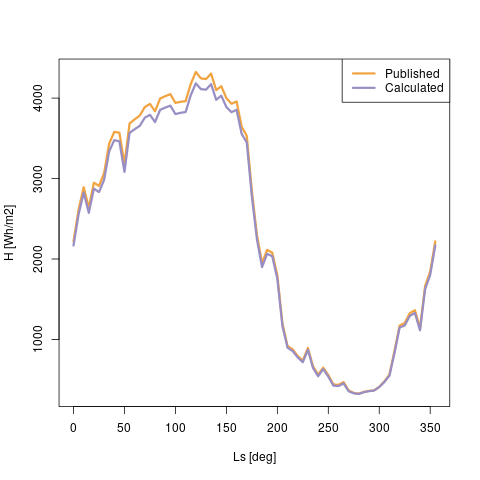
\includegraphics[height=\graphicsHeight]{sections/appendix/A/plots/h-exp-calc-at-vl2-with-beta-22-deg.png}
            \subcaption{Daily variations.}
            \label{fig:sub:comparative-global-insolation-at-vl2-beta-optimal-daily-variations}
    \end{subfigure}\hfill
    \begin{subfigure}[t]{\subfigureWidth}
        \centering
            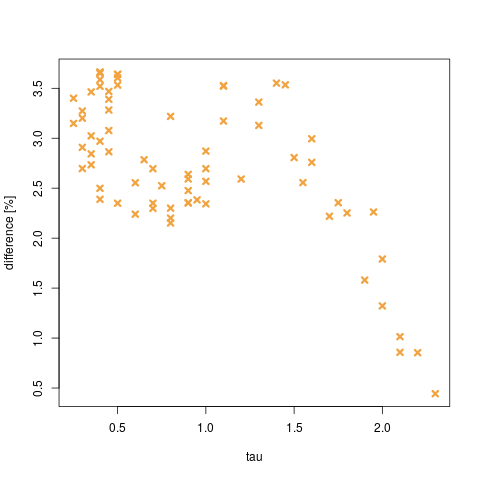
\includegraphics[height=\graphicsHeight]{sections/appendix/A/plots/h-diff-bet-exp-calc-at-vl2-with-beta-22-deg.png}
            \subcaption{Differences as a function of optical depth.}
            \label{fig:sub:comparative-global-insolation-at-vl2-beta-optimal-percentage-differences}
    \end{subfigure}\\[0.8ex]
    \caption{Comparison between published and calculated daily global insolations at \ac{VL2} on a inclined surface with $\beta=\SI{22}{\degree}$.}
    \label{fig:plot:comparative-global-insolation-at-vl2-beta-optimal}
\vspace{-2ex}
\end{figure}
